\documentclass{mnum}
\usepackage{hyperref}
\usepackage[portuguese]{babel}
\title{MNUM -- Exam 2017/18}
\author{Diogo Miguel Ferreira Rodrigues (dmfrodrigues2000@gmail.com)}
% Document
\begin{document}

\setcounter{chapter}{16}
\exam{Exame 2017/18}

\question{Pergunta 1}
A função que pretendo minimizar é
\begin{equation*}
    f(x)=(x-9)^2+x^4
\end{equation*}
Vamos partir do pressuposto de que não sabemos nada sobre a função (exceto que ela é convexa). Assim, vamos utilizar $guess=0$ e passo inicial $h=0.001$, e partir desse ponto para tentar encontrar o mínimo da função.
Os métodos de que dispomos são:
\begin{itemize}
    \item \textbf{Powell}: realizar sucessivas pesquisas lineares (recorrendo a um método ou associação de métodos unidimensional) ao longo de determinados vetores de direção. Adaptado à situação unidimensional, o método de Powell corresponde exatamente ao método ou associação de métodos unidimensional escolhido, pelo que podemos ignorar.
    \item \textbf{Gradiente}: em cada passo, seguir o gradiente multiplicado por um parâmetro variável. Reduzido ao caso unidimensional, é irrelevante (no caso em que o gradiente só determina a direção de pesquisa), ou igual ao método de ajuste quadrático unidimensional.
    \item \textbf{Quádrica}: ajustar a função a uma aproximação de 2º grau, usando o gradiente e a hessiana. Este método é claramente demasiado complexo para as garantias relativamente curtas que dá em termos de tempo de execução, quando comparado com métodos de otimização unidimensional.
    \item \textbf{Método dos terços}: método de redução intervalar, consiste em dividir o intervalo em três partes iguais, e com base no valor da função dos dois valores interiores decidir onde se pode encontrar o mínimo. Menos eficiente do que o método da razão áurea.
    \item \textbf{Método da razão áurea}: semelhante ao método dos terços, mas com razão sendo $\frac{\sqrt{5}-1}{2}$. Mais eficiente por reduzir mais rapidamente o intervalo, além de requerer apenas 1 cálculo da função por passo em vez de 2.
    \item \textbf{Método do ajuste quadrático}: usando três pontos conhecidos da função, determina o mínimo da parábola de melhor ajuste aos três pontos.
    \item \textbf{Enquadramento intervalar de passo constante}: a partir de um guess, obtém um intervalo que contém o mínimo pesquisando de forma linear uma sucessão decrescente até ela começar a aumentar.
    \item \textbf{Enquadramento intervalar de passo variável}: semelhante a passo constante, mas a pesquisa processa-se com passo variável, geralmente a aumentar por um fator de 2.
\end{itemize}
Assim, para resolver este Pergunta, vamos utilizar a seguinte abordagem:
\begin{enumerate}
    \item Realizar enquadramento intervalar do mínimo com passo variável.
    \item Efetuar redução intervalar pelo método da razão áurea, até o intervalo ter amplitude máxima $10^{-10}$.
    \item Realizar um ajuste quadrático para determinar um valor final para o mínimo.
\end{enumerate}
\lstinputlisting[language=Python, caption=Programa 2017E-1 (Python3)]{2017E_1.py}

\question{Pergunta 2}
\lstinputlisting[language=Maxima, caption=Maxima input 2017E-2]{2017E_2.mc}
\lstinputlisting[language=Python, caption=Programa 2017E-2 (Python3)]{2017E_2.py}
\begin{center} \begin{tabular}{l | r | r}
    & Regra Trapézios & Regra Simpson \\ \hline
    $h  $ & 0.12500 & 0.12500 \\
    $h' $ & \textbf{0.06250} & \textbf{0.06250} \\
    $h''$ & \textbf{0.03125} & \textbf{0.03125} \\
    Comprimento do arco $L_1=l  $ & \textbf{11.34629} & \textbf{11.25550} \\
    Comprimento do arco $L_2=l' $ & \textbf{11.27778} & \textbf{11.25495} \\
    Comprimento do arco $L_3=l''$ & \textbf{11.26063} & \textbf{11.25491} \\
    Quociente de convergência $QC$ & \textbf{3.99394} & \textbf{15.85798} \\
    Erro estimado $\varepsilon''$ & \textbf{-0.00572} & \textbf{-0.00000}
\end{tabular} \end{center}

\question{Pergunta 3}
\questionitem{Item a}
\lstinputlisting[language=Maxima, caption=Maxima input 2017E-3.1]{2017E_3_1.mc}
\begin{center} 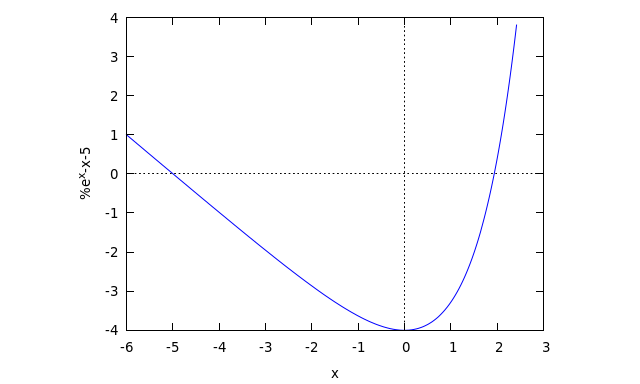
\includegraphics[scale=0.5]{2017E_3_1} \end{center}
Dado que a função é contínua, os seguintes argumentos são suficientes para justificar os intervalos das raízes.
\begin{itemize}
    \item A 1ª raiz pertence ao intervalo $x_1 \in [-6,-4]$, em que a função é monótona decrescente e passa de positiva $f(-6)=1.00248$ para negativa $f(-4)=-0.98168$
    \item A 2ª raiz pertence ao intervalo $x_2 \in [1,3]$, em que a função é monótona crescente e passa de negativa $f(1)=-3.28172$ para positiva $f(3)=12.08554$
\end{itemize}

\questionitem{Item b}
\lstinputlisting[language=Maxima, caption=Maxima input 2017E-3.2]{2017E_3_2.mc}
\begin{center} 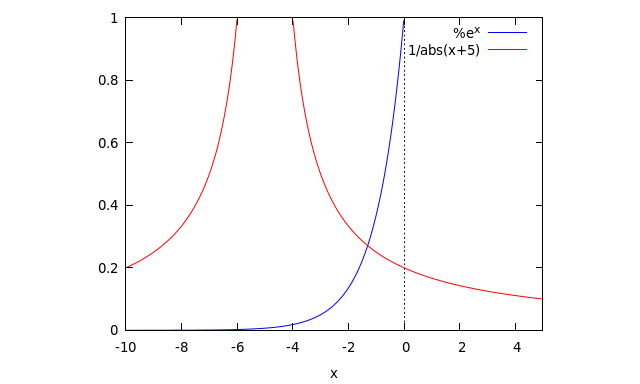
\includegraphics[scale=0.5]{2017E_3_2} \end{center}
Para $x \leq -5$, a fórmula 2 devolve um valor complexo, pelo que iremos considerar como importante a parte da fórmula 2 em que $x > -5$.
Pelo critério $|g'(x)|<1$:
\begin{enumerate}
    \item Converge em aproximadamente $(-\infty, 0)$. Como $|g_1'(x)|<1$ no intervalo da 1ª raiz $x_1 \in [-6,-4]$, a fórmula 1 converge para $x_1$.
    \item Converge em aproximadamente $(-4,+\infty)$. Como $|g_2'(x)|<1$ no intervalor da 2ª raiz $x_2 \in [1,3]$, a fórmula 2 converge para $x_2$.
\end{enumerate}
Analisando a fórmula 1, conclui-se que $x=x_2$ é um ponto de equilíbrio.\\ 
Fazendo um estudo exploratório no Maxima,
\begin{enumerate}
    \item Converge para $x_1=-4.99322$ em $(-\infty, x_2)$, diverge positivamente em $(x_2, +\infty)$, e mantém-se em equilíbrio instável em $x=x_2$.
    \item Converge para $x_2=1.93685$ em $(-5, +\infty)$.
\end{enumerate}

\questionitem{Item c}
Pela alínea anterior, concluímos que a fórmula 1 não é adequada para a determinação por convergência iterativa da raiz $x_2$ (dado que é um ponto de equilíbrio instável, que poderia ser determinado com outro tipo de análise). Assim, das fórmulas dadas sobra apenas a fórmula 2.\par
Em termos de métodos não-intervalares para encontrar soluções de equações, a única alternativa a Picard-Peano lecionada na UC é o método de Newton. Também conhecido como método da tangente, consiste em, a partir do valor anterior $x_{n-1}$, traçar uma reta tangente à função e que passa em $(x_{n-1}, f(x_{n-1}))$, e tomar como valor melhorado $x_n$ a abcissa da interseção dessa reta com o eixo das abcissas.
\lstinputlisting[language=Maxima, caption=Maxima input 2017E-3.3]{2017E_3_3.mc}
\begin{center} 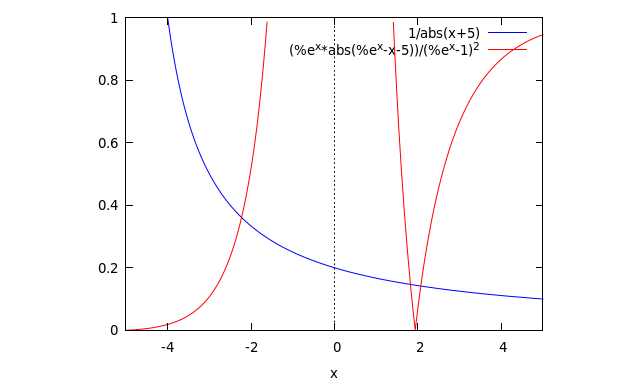
\includegraphics[scale=0.5]{2017E_3_3} \end{center}
Através do gráfico, podemos concluir que a fórmula 3 converge para $x_2$ em aproximadamente $(1.43, +\infty)$, dado que $|g_3'(x)|<1$ na vizinhança de $x_2$ (e, já agora, que converge para $x_1$ em aproximadamente $(-\infty, -1.63)$ dado que no intervalo da 1ª raiz $x_1 \in [-6,-4]$ se verifica $|g_3'(x)|<1$).
\begin{center} 
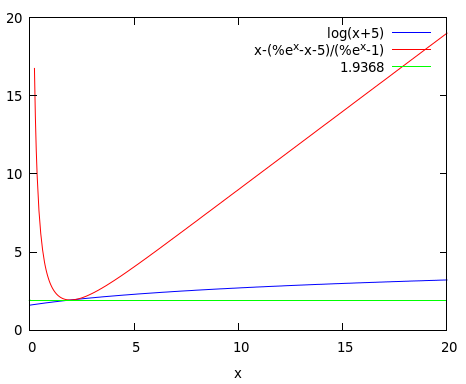
\includegraphics[scale=0.45]{2017E_3_3_02}
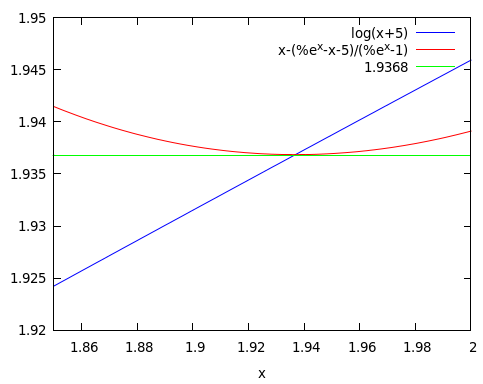
\includegraphics[scale=0.45]{2017E_3_3_03}
\end{center}
Além disso, (assumindo que o guess inicial se encontra na zona de convergência das fórmulas 2 e 3), analisando os gráficos acima podemos concluir que:
\begin{itemize}
    \item A fórmula 2 converge mais rapidamente do que a fórmula 3 quando o valor atual $x_n$ é distante da solução $x_2$, dado que o valor de $g_2(x)$ (azul) é desde logo muito mais próximo de $x_2$ do que $g_3(x)$ (vermelho) quando $x$ é positivo e grande.
    \item A fórmula 3 converge mais rapidamente do que a fórmula 2 quando o o valor atual $x_n$ é já próximo da solução $x_2$, dado que $g_3(x)$ é mais próximo de $x_2$ do que $g_2(x)$ na vizinhança de $x_2$.
\end{itemize}
Nas implementações, usei como critério de paragem para ambas as fórmulas o erro relativo entre iterações consecutivas de $10^{-10}$.
\lstinputlisting[language=Python, caption=Programa 2017E-3.3 (Python3)]{2017E_3_3.py}
Os resultados empíricos apoiam as conclusões "teóricas":
\begin{itemize}
    \item Com guess $x_0=20$, a fórmula 3 parou ao fim de 24 iterações, enquanto a fórmula 2 parou ao fim de apenas 14 iterações.
    \item Com guess $x_0=1.9$ a fórmula 2 parou ao fim de 11 iterações, enquanto a fórmula 3 parou ao fim de apenas 4 iterações.
\end{itemize}
Em conclusão, dado que já sabíamos por várias vias o valor aproximado da 2ª raiz (cerca de 1.93), neste caso a melhor solução seria utilizar o método de Newton com esse guess.

\question{Pergunta 4}
\lstinputlisting[language=Python, caption=Programa 2017E-4 (Python3)]{2017E_4.py}
\begin{center}
    \begin{minipage}[c]{0.5\textwidth}
        \questionitem{Item a}
        \begin{center} \begin{tabular}{c | r | r | r}
            Iteração & $t$ & $C$ & $T$ \\ \hline
            0        & 0.00000 & \textbf{2.50000} & \textbf{25.00000} \\
            1        & \textbf{0.25000} & \textbf{1.87605} & \textbf{43.09357} \\
            2        & 0.50000 & \textbf{1.40778} & \textbf{54.25499}
        \end{tabular} \end{center}
    \end{minipage}%
    \begin{minipage}[c]{0.5\textwidth}
        \questionitem{Item b}
        \begin{center} \begin{tabular}{c | r | r | r}
            Iteração & $t$ & $C$ & $T$ \\ \hline
            0        & 0.00000 & \textbf{2.50000} & \textbf{25.00000} \\
            1        & \textbf{0.25000} & \textbf{1.94782} & \textbf{39.94349} \\
            2        & 0.50000 & \textbf{1.51757} & \textbf{49.70136}
        \end{tabular} \end{center}
    \end{minipage}%
\end{center}
\questionitem{Item c}
\begin{center} \begin{tabular}{c | r || c | r}
    $h' $ & \textbf{0.12500} & $T_{h' }$ & \textbf{51.77067} \\
    $h' $ & \textbf{0.06250} & $T_{h' }$ & \textbf{50.69205} \\
          &                  & Quociente de convergência & \textbf{2.30325} \\
          &                  & Erro absoluto estimado & \textbf{-1.07861}
\end{tabular} \end{center}

\question{Pergunta 5}
\lstinputlisting[language=Python, caption=Programa 2017E-5 (Python3)]{2017E_5.py}

\end{document}
